\documentclass[journal,comsoc]{IEEEtran}
\usepackage[T1]{fontenc}% optional T1 font encoding

\usepackage{ifpdf}
\usepackage{cite}
\ifCLASSINFOpdf
  \usepackage[pdftex]{graphicx}
\else
  \usepackage[dvips]{graphicx}
\fi
\usepackage{amsmath}
\interdisplaylinepenalty=2500
\usepackage[cmintegrals]{newtxmath}
\usepackage{bm}
\usepackage{algorithmic}
\usepackage{array}
\ifCLASSOPTIONcompsoc
  \usepackage[caption=false,font=normalsize,labelfont=sf,textfont=sf]{subfig}
\else
  \usepackage[caption=false,font=footnotesize]{subfig}
\fi
%\usepackage{fixltx2e}
%\usepackage{stfloats}
\ifCLASSOPTIONcaptionsoff
  \usepackage[nomarkers]{endfloat}
 \let\MYoriglatexcaption\caption
 \renewcommand{\caption}[2][\relax]{\MYoriglatexcaption[#2]{#2}}
\fi
\usepackage{url}
\usepackage{hyperref}
% correct bad hyphenation here
\hyphenation{op-tical net-works semi-conduc-tor}

\newcommand{\J}{\textbf{J}}

\begin{document}
\title{Temporal-Spatial Depth Map Based Hand Pose Estimation}

\author{{Anonymous}% <-this % stops a space
\thanks{Anonymous}}

% The paper headers
\markboth{Journal of \LaTeX\ Class Files,~Vol.~14, No.~8, August~2015}%
{Shell \MakeLowercase{\textit{et al.}}: Bare Demo of IEEEtran.cls for IEEE Communications Society Journals}

% make the title area
\maketitle

\begin{abstract}
Abstract
\end{abstract}

% Note that keywords are not normally used for peerreview papers.
\begin{IEEEkeywords}
Hand pose estimation, Recurrent Network, Mixture of Experts.
\end{IEEEkeywords}


% For peer review papers, you can put extra information on the cover
% page as needed:
\ifCLASSOPTIONpeerreview
\begin{center} \bfseries EDICS Category: 3-BBND \end{center}
\fi
%
% For peerreview papers, this IEEEtran command inserts a page break and
% creates the second title. It will be ignored for other modes.
\IEEEpeerreviewmaketitle


\section{Introduction}\label{sec:introduction}
\IEEEPARstart{H}{and} pose estimation is an essential problem in computer vision, and plays an pivotal
role in vision application such as human-computer interface (HCI), augmentation reality (AR)~\cite{barsoum2016articulated}. So
far, there are a plenty of researches on this topic~\cite{guo2017region, quach2016depth, ge2017_3D,
wan2017crossing}, and major progresses have been made thanks to the improvement in deep learning
and low cost depth sensors. Nevertheless, hand is the most complex human part to analyse, and the
problem is still far from solved, it is still difficult to estimate hand pose in the practical scene
owing to several reasons. (1) the image quality is poor because of the commercial depth sensor, (2)
hand is a articulated object with high degrees of freedom (DoFs), the fingers are similar with each
other and apt to occlude each other, (3) in a real scenario, the application must process the depth
image real-timely, which increase the difficulty for estimation.

In general, the purpose of hand pose estimation is to estimate the 3D location of joints. Most existing
methods concentrate on the hand spatial structure modelling, such as the nodes in regression decision
forest and sparated stage in cascaded CNN, while ignoring the coherence between the current frame and
the previous frame. For instance, when we humans find the joint locations, we usually search in the
patches around the previous frame's joints. It reveals that the previous frame's pose provides abundant
information for pose estimation. However, many existing methods~\cite{oberweger2015hands, ge2017_3D} learn
the mapping from depth image or 3D voluetric representation to the hand pose. Some methods
~\cite{sun2015cascaded, ye2016spatial} explicitly model the hierarchical hand structure in addition. In
practice, depth images are in selected from videos, and video has time-varying dynamic properties.

Motivated by the oberservation above, we propose a method focus on the spatial structure as well as
temporal information. The different viewpoint for solving the problem is modelled as different part in
our method. Figure.~\ref{fig:architecture} shows a holistic illustration for our approach. The first 
part is denoted as \emph{Spatial Network} in this paper, which learns the mapping to hand pose from 
spatial information. \emph{Spatial Network} works on a single depth image, with the depth image and 
corresponding sliced 3D volumetric representation input into the network, spatial information extracted
hierarchically improve the performance of pose estimation. The second part is denoted as \emph{Temporal Network}. 
This network pay attention to the time 



\begin{figure}[t]
    \centering
    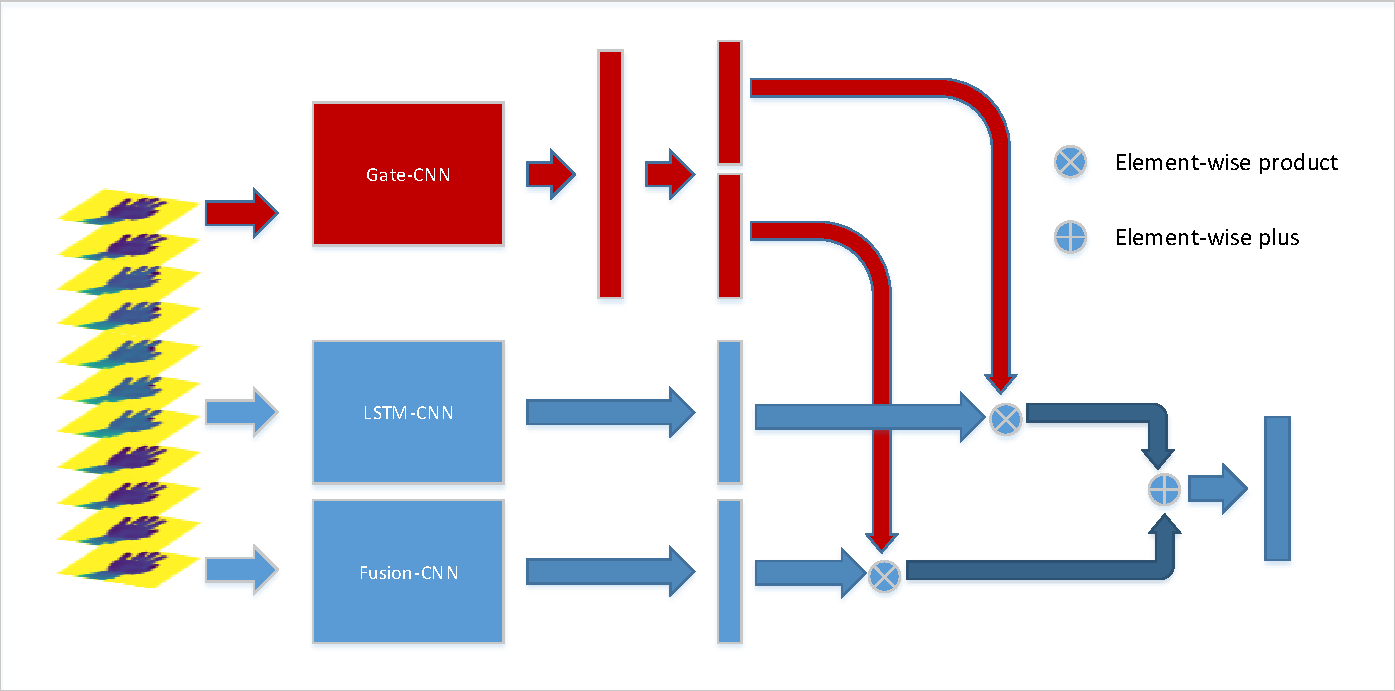
\includegraphics[width=1\linewidth]{src/network/architecture.pdf}
    \caption{The overview of architecture. The red branch is the \emph{Gate Network}, the blue
    branch is the expert networks. \emph{Temporal Network} extract the correlated features considering
    the sequentiality of input images and \emph{Spatial Network} employ the Deeply-fusion framework to
    fuse depth image and 3D volumetric representations, \emph{Gate Network} weights the prediction
    from each expert.}
\label{fig:architecture}
\end{figure}

The estimation network is evaluated on two public datasets. Due to the practicability, the network
could run in in real-time on the GPU and achieve the comparable or better results than state-of-art methods.
We summary our contribution in the following three folds:
\begin{itemize}
  \item
  We integrate features from depth map and sliced 3D volumetric representation for hand pose
  estimation by deep fusion network. The experiment reveals that 3D volumetric representation
  benefits the hand pose estimation.
  \item
  We model the coherence among frames by LSTM, and implement a hand pose
  estimation system with an eye to accuracy, efficiency, robustness and stability
  simultaneously.
  \item
  We evaluate our approach on two public datasets (e.g. NYU and ICVL), and get the
  comparable or better results than state-of-art methods.
\end{itemize}

% needed in second column of first page if using \IEEEpubid
%\IEEEpubidadjcol

%-------------------------------------------------------------------------
\section{Related Work}\label{sec:related work}
\subsection{Hand Pose Estimation}


%------------------------------------------------------------------------
\section{Hand Pose Estimation}\label{sec:hand pose estimation}
In this paper, we concentrate on the efficient 3D hand pose estimation from the depth images and
introduce a robust spatial-temporal hand pose estimation approach. In the natural scene, the camera
capture the consecutive frames and hand is contained in the frame.
The hand pose in the between frames is highly correlated. Inspired by the hand pose
tracking~\cite{quach2016depth}, we embed Long Short Time Memory (LSTM) into a \emph{Temporal Network}
to extract features considering the sequentiality. Recurrent LSTM encode the original sequential
features into a correlated features for estimation. Furthermore, the spatial information of hand is
important, many approaches focus on tree structured skeleton of hand to address this problem (e.g.
~\cite{li20153d, wan2016direction, ye2016spatial}). And 3D volumetric representation could well reserve
the spatial information~\cite{deng2017hand3d} for solving pose estimation in 3D. We employ the
Deeply-fusion framework ~\cite{wang2016deeply} to fuse depth image and 3D volumetric representations,
which is called \emph{Spatial Network}. \emph{Temporal Network} and \emph{Spatial Network} predict
hand joint locations based on different features, which is the expert in the Mixture of Experts
(MoE). In MoE, the different experts give out their predictions and \emph{Gate Network} weights the
predictions.



% In this section, we introduce our method for hand pose estimation. Figure
% ~\ref{fig:architecture} shows the entire architecture. Aspired by Mixture of Experts
% ~\cite{jacobs1991adaptive}, network is composed of two parts: \emph{Gate Network} and
% \emph{Expert Networks}, we use a \emph{Gate Network} to control two expert networks.
% Each expert predicts the 3D pose given the input image, the \emph{Gate Network} weights
% the prediction from each expert. The experts concentrate on different information.
% \emph{Temporal Network} takes temporal context into account between the consecutive frames.
% \emph{Spatial Network}, thinking over spatial information, fuses the features from depth
% map and 3D volumetric representation.

% The \emph{Temporal Network} and \emph{Spatial Network} we employed are discussed in Section
% ~\ref{sec:temporal netowork} and Section~\ref{sec:spatial network}, and \emph{Gate Network} is
% discussed in Section~\ref{sec:gate network}.

\subsection{Problem Analysis}\label{sec:problem analysis}
% prepare the notation for problem
Our objective is to predict the 3D hand joint locations from a depth image containing a hand,
the locations are represented as a set of keypoints. Here we give some notations about the
problem. We denote a depth image as $I$, and the corresponding hand pose is
$\J=\{\textbf{j}_i\}_i^n$ with $\textbf{j}_i=(x_i,y_i,z_i)$ representing a 3D position of a
joint in the depth image $I$. And $n$ is the number of joints, it is different between plenties
of datasets (e.g. $n=36$ for NYU, $n=16$ for ICVL).


\subsection{Temporal Network}\label{sec:temporal netowork}
\begin{figure}[t]
    \centering
    \subfloat[Baseline]{
        \label{fig:baseline network}
        \begin{minipage}[t]{116pt}
            \centering
            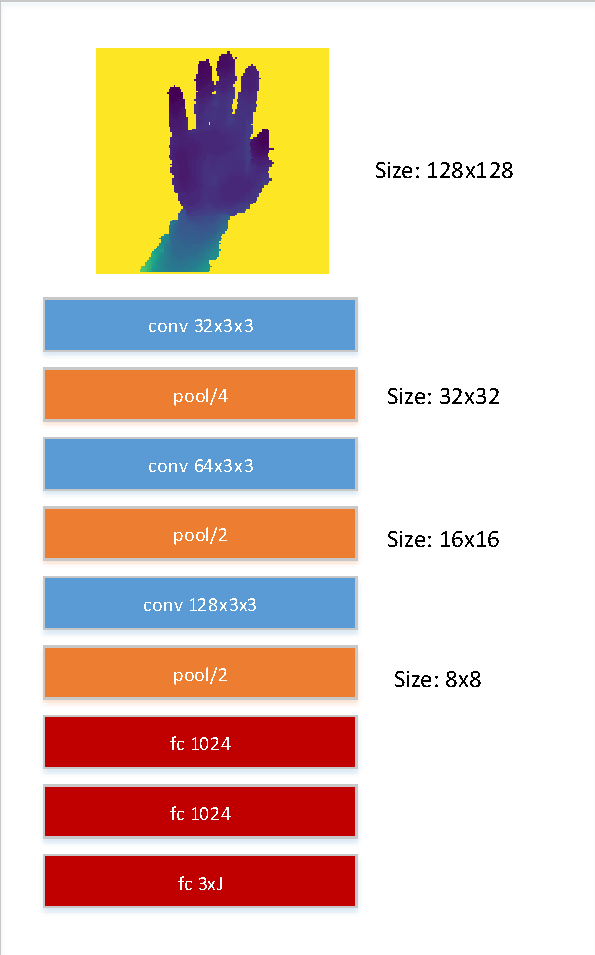
\includegraphics[width=1\linewidth]{src/network/baseline.pdf}
        \end{minipage}
    }
    \subfloat[Temporal Network.]{
        \label{fig:temporal network}
        \begin{minipage}[t]{110pt}
            \includegraphics[width=1\linewidth]{src/network/temporal.pdf}
        \end{minipage}
    }
\caption{\emph{Baseline} and \emph{Temporal network}. In \emph{Baseline}, activation
function is relu which is follow by convolution layer and fully connected layer, and dropout is
adopted to resist overfitting. In \emph{Temporal Network}, the parameters in previous layers are
borrowed from \emph{Baseline}, lstm layer and last fully connected layer are trained when
the input is a sequence of images.}
\label{fig:baseline and lstm network}
\end{figure}

As we know, the hand poses between successive frames are correlated (e.g. when grabbing, the joints
on fingers are most likely to be closer). Currently, an Recurrent Neural Network (RNN) with Long
Short-Term Memory (LSTM) units~\cite{zaremba2014learning} is widely used because they are expressive
and easy to train. The LSTM network is mostly used for modeling the long term temporal correspondence.
\cite{quach2016depth} use RNN regress the joint location straight forward, and training CNN and RNN
simultaneously. We do several modifications to extract robust features and have better result with
temporal information.

As is shown in Figure~\ref{fig:temporal network}, a sequence of frames $\{I_1, I_2, \dots, I_N\}$ is
taken as input and give out the estimated pose. Considering the $t$-th depth image $I_t$, the image
flow through the convolution network and the feature extracted is denoted as follows,
\begin{equation}
\phi(I_t)=f_{\theta_c}(pre(I_t))
\end{equation}
where $f_{\theta_c}(\cdot)$ is a convolutional network with parameters $\theta_c$ and
$pre(\cdot)$ is the preprocessing to crop out the hand. The preprocessing step is declared
in Section.~\ref{sec:experiments}. The feature is fed into LSTM and LSTM output its hidden
state as new feature,
\begin{equation}
h_t=f_{\theta_l}(h_{t-1}, \phi(I_t))
\end{equation}
where $f_{\theta_l}$ is the parameters in LSTM cell. The new features and original features
are concatenated then fed into the last fully connected layer and network give out the prediction.

In the training stage, CNN network for extracting features is pre-trained. In Figure.
~\ref{fig:baseline network}, the LSTM layer is replaced by a fully connected layer.
With the parameters in CNN is fixed, we train LSTM and last layer solely.

\subsection{Spatial Network}\label{sec:spatial network}
According to the discussion in \cite{supancic2015depth, deng2017hand3d, ge2017_3D}, 3D
volumetric representation benefits the hand pose estimation. However, due to the high
cost of 3D convolution, the input is mostly small such as 32x32x32
~\cite{deng2017hand3d, ge2017_3D}, which results in "details lost". We employ an eclectic
solution, the background is omitted in our 3D representation, and the space is sliced
into 8 layers to preserve more details. The exemplar is shown in Figure.
~\ref{fig:spatial network}.

The 3D volumetric representation keep the structure of hand, we can clearly find all
finger tips in the first layer, with a low cost for memory at the mean time. Nevertheless,
the depth information is deprecated in our 3D volumetric representation, it makes harder
to estimate the depth of hand joints. To obtain the structure information and depth
information simultaneously, we combine these information from depth image and 3D volumetric
representation together. In Figure.~\ref{fig:spatial network}, we employ a Deep-Fusion
framework~\cite{chen2016multi} to fuse the features and named as \emph{Spatial Network}.

In the \emph{Spatial Network}, the different features are fused together hierarchically.
which could be expressed as:
\begin{equation}\label{eq:deep fusion}
\begin{aligned}
&f_0 = f_{depth} \oplus f_{3D} \\
&f_l = \textbf{H}_l^{depth}(f_{l-1}) \oplus \textbf{H}_l^{3D}(f_{l-1}) \\
&\forall l=1, \dots , L
\vspace{1em}
\end{aligned}
\end{equation}
The $\oplus$ is element-wise mean, $f_{depth}$ and $f_{3D}$ are the features output from
two pooling layers, $\textbf{H}$ is the transformation for features,
$l$ is the index for layer.

Owing to the several fully connected layers, the network tends to overfitting, so we use
an auxiliary loss as the regularization as well as dropout. In Figure.~\ref{fig:spatial network},
every fully connected layer is followed by a dropout layer, the nodes are dropout randomly
with 30\% probability. For the purpose of obtaining more representative capability for each input
, the auxiliary paths are added in training stage. As shown in the green boxes, layers in the
auxiliary paths are same as the main network, the layers connected by the blue dotted line
share parameters. And in the training stage, the total losses are composed by three losses,
i.e. three regression loss in auxiliary paths and main network. When testing, the auxiliary
pathes are removed.
\begin{figure*}[t]
    \centering
    \includegraphics[width=0.5\linewidth]{src/network/spatial.pdf}
    \caption{Spatial Network}
\label{fig:spatial network}
\end{figure*}

\subsection{Gate Network}\label{sec:gate network}
The foregoing \emph{Temporal Network} and \emph{Spatial Network} stand in the different views
for estimating the joints, we name the predictions as $\J_{temp}$ and $\J_{spa}$. To improve
the performance, we want to ensemble their advantages for last prediction. Jacob. et al
proposed Mixture of Experts (MoE) ~\cite{jacobs1991adaptive} for adaptively integrating
different regressors.

\emph{Gate Network} weights two predictors, and give out the last prediction according to
the weights of predictions as follow:
\begin{equation}\label{eq:gate network}
\centering
\textbf{J}_{out} = \textbf{g}_1 \J_{temp} + \textbf{g}_2 \J_{spa}
\end{equation}
where $\textbf{g}_1$ and $\textbf{g}_2$ are the weight of \emph{Gate Network}. The final prediction
$\textbf{J}_{out}$ is estimated as the weighted sum of each prediction.

Because \emph{Temporal Network} considers the temporal information and \emph{Spatial Network}
extracts the spatial information, mixture of experts infer the hand joint location based on
spatial-temporal features. Comparing with baseline network, \emph{Gate Network} outputs higher
dimension weights, so we employ a more complex network by increasing the size of convolution kernels.
Specifically, we double the parameters in the gate network than the baseline network, and employ Dropout~\cite{srivastava2014dropout} after
the fully connected layer to prevent overfitting (the detail network is shown in Appendix~\ref{sec:gate network architecture}).


%\begin{figure}[t]
%    \centering
%    \includegraphics[width=1\linewidth]{}
%    \caption{Gating Network}
%\label{fig:gating network}
%\end{figure}


%-------------------------------------------------------------------------
\section{Experiments}\label{sec:experiments}
In this section, we evaluate our approach on two public datasets, NYU~\cite{tompson2014real}
and ICVL~\cite{tang2014latent}, for comparison with the state-of-art methods. In addition, we
do ablation experiments and analyse the performance of each component. We first describe our
experiment setting.

\subsection{Experiment Setting}\label{sec:experiment setting}
\subsubsection{Datasets}\label{sec:datasets}
NYU dataset is composed of 72K training and 8K testing images captured by PrimeSense. The
annotation is obtained by model-based tracking with a Particle Swarm Optimization processing.
This dataset is challenge because of its wider pose variation and noisy image as well as limited
annotation accuracy. ICVL dataset is smaller than NYU dataset, contains 22K frames for training
and 1.6K frames for testing. The resolution of images is only 320x240 and captured by Creative Interactive
Gesture Camera. The scale of image is small and the discrepancies between training and testing is
large, these makes the estimation hard. In the test sequences, the finger movement is more evident
than the train sequences.

\subsubsection{Evaluation Metrics}\label{sec:evaluation metrics}
The evaluation follows the standard metrics proposed in~\cite{tompson2014real}, including a
plot of the percentage of test samples given a maximum distance from ground truth and average
distance error (in mm). There are totally 36 annotated joints in NYU dataset, but we only
evaluate a subset of 14 joints for a fair comparison. In addition to ICVL dataset
, we evaluate 16 annotated joints for comparison.

\subsubsection{Implementation Details}\label{sec:implementation}
We implement the training and testing with Caffe\cite{jia2014caffe}. The segmentation step
follows~\cite{oberweger2015hands} to extract a cube from the depth image, and the cube is
resized to a 128x128 depth image with the depth value normalized to [-1, 1]. Moreover, we
augment the dataset by random rotation.

The three components of network are trained separately. The baseline network is pre-trained for
\emph{Temporal Network} and \emph{Spatial Network} with Adam, we set the learning rate as 1e-3
and train the network for 100,000 iterations, the learning rate is divided by 10 every 20,000
iterations and the mini-batch is set as 128. \emph{Spatial Network} is trained from scratch,
with the same setting as baseline network. \emph{Temporal Network} trained based on the baseline
network with the parameters fixed, and the configuration is same except that we only train the
network for 50,000 iterations.  To train the \emph{Gate Network}, the parameters are all fixed
but the parameters in gate branch and the network is trained for 50,000 iterations. Our training
takes place on machines equipped with a 12GB Titan X GPU and 64GB memory.

\subsection{Experiment Results}\label{sec:experiment results}
\subsubsection{Comparison with State-of-art}\label{sec:comparison}
We compare our approach with several CNN based hand pose estimation method. We compare with
four methods~\cite{tompson2014real, oberweger2015hands, oberweger2015training, zhou2016model}
on NYU dataset, and compare with two methods~\cite{oberweger2015hands, zhou2016model} on ICVL
dataset. The mean error of different methods is shown in Tab.~\ref{tab:mean error NYU} and Tab.
~\ref{tab:mean error ICVL} as well as average error shown in Figure.~\ref{fig:Qualitative result NYU}.

\begin{table}[htbp]\footnotesize
\centering
    \begin{tabular}{|c|c|c|c|c|c|}
    \hline
    Methods        &\cite{tompson2014real} &\cite{oberweger2015hands} &\cite{oberweger2015training} &\cite{zhou2016model} &Ours\\
    \hline
    Mean Error(mm) &21.0                   &20.8                      &15.9                         &16.9                 &14.8\\
    \hline
\end{tabular}
\vspace{1em}
\caption{Comparison between our approach and state-of-art methods for mean error.}
\label{tab:mean error NYU}
\end{table}

\begin{table}[htbp]\footnotesize
\centering
    \begin{tabular}{|c|c|c|c|}
    \hline
    Methods        &\cite{oberweger2015hands} &\cite{zhou2016model} &Ours\\
    \hline
    Mean Error(mm) &0                      &0                       &0\\
    \hline
    \end{tabular}
\vspace{1em}
\caption{Comparison between our approach and state-of-art methods for mean error.}
\label{tab:mean error ICVL}
\end{table}

\begin{figure*}[t]\footnotesize
\centering
    \subfloat[]{
        \label{fig:comparison NYU}
        \begin{minipage}[t]{200pt}
            \centering
            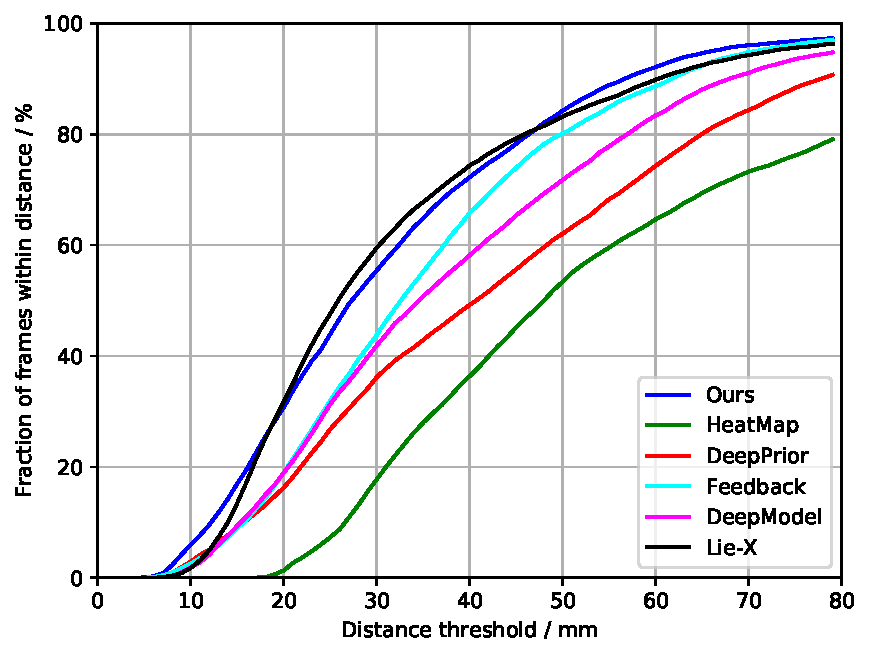
\includegraphics[width=1\linewidth]{src/experiment/eval/NYU_comparison/comparison_frameswithin.pdf}
        \end{minipage}
    }
    \subfloat[]{
        \label{fig:joint mean NYU}
        \begin{minipage}[t]{260pt}
            \centering
            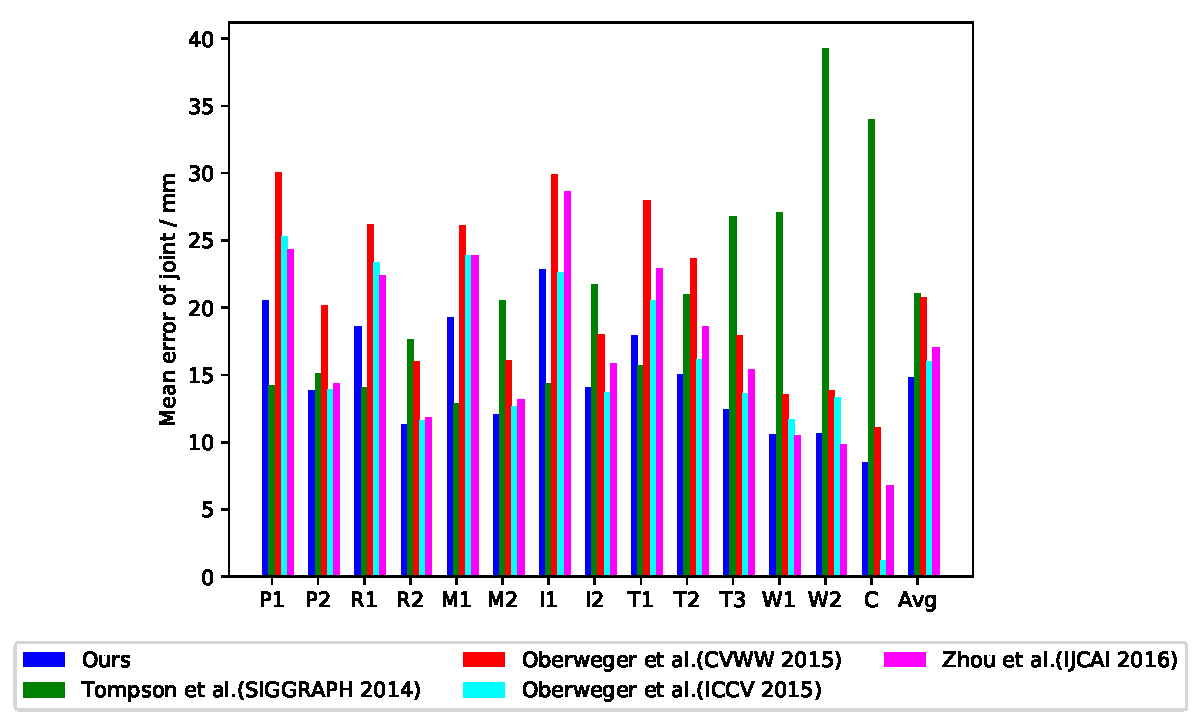
\includegraphics[width=1\linewidth]{src/experiment/eval/NYU_comparison/comparison_joint_mean.pdf}
        \end{minipage}
    }
    \caption{Qualitative results for NYU dataset.}
    \label{fig:Qualitative result NYU}
\end{figure*}
\subsubsection{Ablation}\label{sec:ablation}
To show the effects of different parts in mixed network, we do the ablation experiments. We
show the test result on NYU and ICVL dataset in Figure.~\ref{fig:Qualitative result ablation}.

\begin{figure*}[t]\footnotesize
\centering
    \subfloat[]{
        \label{fig:ablation NYU}
        \begin{minipage}[t]{200pt}
            \centering
            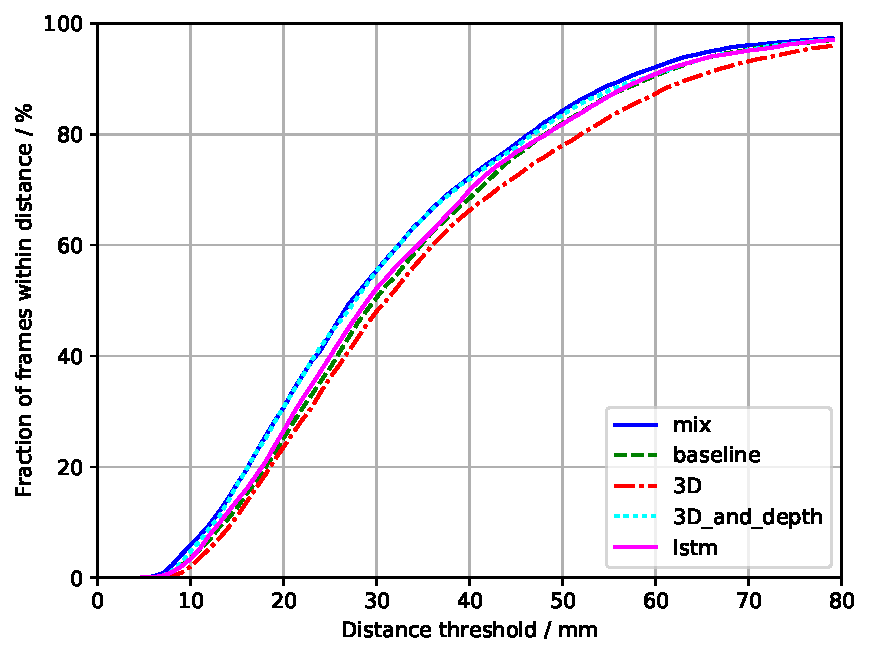
\includegraphics[width=1\linewidth]{src/experiment/eval/NYU_ablation/ablation_frameswithin.pdf}
        \end{minipage}
    }
    \subfloat[]{
        \label{fig:ablation joint mean NYU}
        \begin{minipage}[t]{180pt}
            \centering
            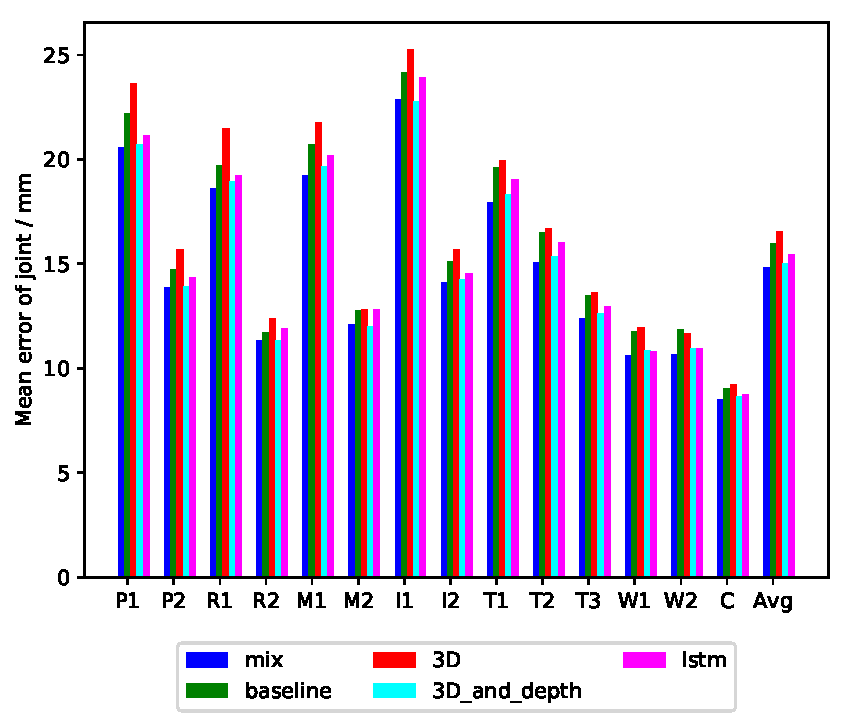
\includegraphics[width=1\linewidth]{src/experiment/eval/NYU_ablation/ablation_joint_mean.pdf}
        \end{minipage}
    }
    \caption{Qualitative results for ablation experiments.}
    \label{fig:Qualitative result ablation}
\end{figure*}

\section{Conclusion}\label{sec:conclusion}
The conclusion goes here.

% An example of a floating figure using the graphicx package.
% Note that \label must occur AFTER (or within) \caption.
% For figures, \caption should occur after the \includegraphics.
% Note that IEEEtran v1.7 and later has special internal code that
% is designed to preserve the operation of \label within \caption
% even when the captionsoff option is in effect. However, because
% of issues like this, it may be the safest practice to put all your
% \label just after \caption rather than within \caption{}.
%
% Reminder: the "draftcls" or "draftclsnofoot", not "draft", class
% option should be used if it is desired that the figures are to be
% displayed while in draft mode.
%
%\begin{figure}[!t]
%\centering
%\includegraphics[width=2.5in]{myfigure}
% where an .eps filename suffix will be assumed under latex,
% and a .pdf suffix will be assumed for pdflatex; or what has been declared
% via \DeclareGraphicsExtensions.
%\caption{Simulation results for the network.}
%\label{fig_sim}
%\end{figure}

% Note that the IEEE typically puts floats only at the top, even when this
% results in a large percentage of a column being occupied by floats.


% An example of a double column floating figure using two subfigures.
% (The subfig.sty package must be loaded for this to work.)
% The subfigure \label commands are set within each subfloat command,
% and the \label for the overall figure must come after \caption.
% \hfil is used as a separator to get equal spacing.
% Watch out that the combined width of all the subfigures on a
% line do not exceed the text width or a line break will occur.
%
%\begin{figure*}[!t]
%\centering
%\subfloat[Case I]{\includegraphics[width=2.5in]{box}%
%\label{fig_first_case}}
%\hfil
%\subfloat[Case II]{\includegraphics[width=2.5in]{box}%
%\label{fig_second_case}}
%\caption{Simulation results for the network.}
%\label{fig_sim}
%\end{figure*}
%
% Note that often IEEE papers with subfigures do not employ subfigure
% captions (using the optional argument to \subfloat[]), but instead will
% reference/describe all of them (a), (b), etc., within the main caption.
% Be aware that for subfig.sty to generate the (a), (b), etc., subfigure
% labels, the optional argument to \subfloat must be present. If a
% subcaption is not desired, just leave its contents blank,
% e.g., \subfloat[].


% An example of a floating table. Note that, for IEEE style tables, the
% \caption command should come BEFORE the table and, given that table
% captions serve much like titles, are usually capitalized except for words
% such as a, an, and, as, at, but, by, for, in, nor, of, on, or, the, to
% and up, which are usually not capitalized unless they are the first or
% last word of the caption. Table text will default to \footnotesize as
% the IEEE normally uses this smaller font for tables.
% The \label must come after \caption as always.
%
%\begin{table}[!t]
%% increase table row spacing, adjust to taste
%\renewcommand{\arraystretch}{1.3}
% if using array.sty, it might be a good idea to tweak the value of
% \extrarowheight as needed to properly center the text within the cells
%\caption{An Example of a Table}
%\label{table_example}
%\centering
%% Some packages, such as MDW tools, offer better commands for making tables
%% than the plain LaTeX2e tabular which is used here.
%\begin{tabular}{|c||c|}
%\hline
%One & Two\\
%\hline
%Three & Four\\
%\hline
%\end{tabular}
%\end{table}


% Note that the IEEE does not put floats in the very first column
% - or typically anywhere on the first page for that matter. Also,
% in-text middle ("here") positioning is typically not used, but it
% is allowed and encouraged for Computer Society conferences (but
% not Computer Society journals). Most IEEE journals/conferences use
% top floats exclusively.
% Note that, LaTeX2e, unlike IEEE journals/conferences, places
% footnotes above bottom floats. This can be corrected via the
% \fnbelowfloat command of the stfloats package.

% if have a single appendix:
%\appendix[Proof of the Zonklar Equations]
% or
%\appendix  % for no appendix heading
% do not use \section anymore after \appendix, only \section*
% is possibly needed

% use appendices with more than one appendix
% then use \section to start each appendix
% you must declare a \section before using any
% \subsection or using \label (\appendices by itself
% starts a section numbered zero.)
%


\appendices
\section{Gate Network Architecture}\label{sec:gate network architecture}
Appendix one text goes here.


% use section* for acknowledgment
\section*{Acknowledgment}


The persons would like to thank...


% Can use something like this to put references on a page
% by themselves when using endfloat and the captionsoff option.
\ifCLASSOPTIONcaptionsoff
  \newpage
\fi



% trigger a \newpage just before the given reference
% number - used to balance the columns on the last page
% adjust value as needed - may need to be readjusted if
% the document is modified later
%\IEEEtriggeratref{8}
% The "triggered" command can be changed if desired:
%\IEEEtriggercmd{\enlargethispage{-5in}}

% references section

% can use a bibliography generated by BibTeX as a .bbl file
% BibTeX documentation can be easily obtained at:
% http://mirror.ctan.org/biblio/bibtex/contrib/doc/
% The IEEEtran BibTeX style support page is at:
% http://www.michaelshell.org/tex/ieeetran/bibtex/
%\bibliographystyle{IEEEtran}
% argument is your BibTeX string definitions and bibliography database(s)
%\bibliography{IEEEabrv,../bib/paper}
%
% <OR> manually copy in the resultant .bbl file
% set second argument of \begin to the number of references
% (used to reserve space for the reference number labels box)
\bibliography{wu}
\bibliographystyle{IEEEtran}

% biography section
%
% If you have an EPS/PDF photo (graphicx package needed) extra braces are
% needed around the contents of the optional argument to biography to prevent
% the LaTeX parser from getting confused when it sees the complicated
% \includegraphics command within an optional argument. (You could create
% your own custom macro containing the \includegraphics command to make things
% simpler here.)
%\begin{IEEEbiography}[{\includegraphics[width=1in,height=1.25in,clip,keepaspectratio]{mshell}}]{Michael Shell}
% or if you just want to reserve a space for a photo:

% insert where needed to balance the two columns on the last page with
% biographies
%\newpage

%\begin{IEEEbiographynophoto}{Jane Doe}
%Biography text here.
%\end{IEEEbiographynophoto}

% You can push biographies down or up by placing
% a \vfill before or after them. The appropriate
% use of \vfill depends on what kind of text is
% on the last page and whether or not the columns
% are being equalized.

%\vfill

% Can be used to pull up biographies so that the bottom of the last one
% is flush with the other column.
%\enlargethispage{-5in}



% that's all folks
\end{document}


